% !Mode:: "TeX:UTF-8"
% !TEX program= xelatex
\documentclass[a4paper]{article}
\usepackage{amsmath}
\usepackage{amssymb}
\usepackage{ctex}
%\usepackage{fourier}
%\usepackage{braket}
%\usepackage[european]{circuitikz}
\usepackage{multirow}
\usepackage{float}
\usepackage{graphicx}
\usepackage{geometry}
\geometry{left=2.5cm, right=2.5cm, bottom=2.5cm, top=2.5cm}
%\newcommand*{\rom}[1]{\expandafter\@slowromancap\romannumeral #1@}
\newcommand{\rom}[1]{\textup{\uppercase\expandafter{\romannumeral#1}}}
\newcommand{\parallelsum}{\mathbin{\!/\mkern-5mu/\!}}
\title{\Huge 近代物理实验报告\\\huge 10.1:各向异性磁电阻、巨磁电阻测量}
\author{xy\quad 学号\quad 匡亚明学院}
\date{2019年2月29日}
\begin{document}
\maketitle
\bibliographystyle{unsrt}
%--------main-body------------

\section{引言}
一般所谓磁电阻是指在一定磁场下材料电阻率改变的现象。通常将磁场引起的电阻率变化写成$\Delta\rho = \rho(H) - \rho(0)$,其中$\rho(H)$和$\rho(0)$分别表示在磁场H中和无磁场时的电阻率。磁电阻的大小常表示为
\begin{equation*}
	\text{MR} = \frac{\Delta\rho}{\rho}\times 100\%
\end{equation*}
其中$\rho$可以是$\rho(0)$或$\rho(H)$,MR是magnetoresistivity的缩写。

绝大多数非磁性导体的MR很小,约为$10^{-5}$\%,磁性导体的MR最大为3\%$\sim$5\%,且电阻率的变化与磁场方向与导体中电流方向的夹角有关,即具有各向异性,称之为各向异性磁电阻(AMR)。

1988年,在分子束外延制备的Fe/Cr多层膜中发现MR可达50\%。并且在薄膜平面上,磁电阻是各向同性的。人们把这称之为巨磁电阻(GMR),90年代,人们又在Fe/Cu、Fe/Al、Fe/Ag、Fe/Au、Co/Cu、Co/Cu和Co/Cu等纳米多层膜中观察到了显著的巨磁电阻效应。

1992年人们又发现在非互溶合金(如Fe、Co与Cu、Ag、Au等在平衡态不能形成合金)颗粒膜如Co-Ag、Co-Cu中存在巨磁电阻效应,在液氮温度可达55\%,室温可达到20\%,并且有各向同性的特点。

1994年,人们又发现Fe/Al2O3/Fe隧道结在4.2K的MR为30\%,室温达18\%,之后在其他一些铁磁层/非铁磁层/铁磁层隧道结中亦观察到了大的磁电阻效应,人们将此称为隧道结磁电阻(TMR)。目前MR室温达24\%的TMR材料已制成,用TMR材料已制成计算机硬盘读出磁头,其灵敏度比普通MR磁头高10倍,比GMR磁头高数倍。

20世纪90年代后期,人们在掺碱土金属稀土锰氧化物中发现MR可达$10^3\%\sim 10^6\%$,称之为庞磁电阻(简记为CMR)。目前锰氧化物CMR材料的磁电阻饱和磁场较高,降低其饱满和场是将之推向应用的重要研究课题。
利用磁电阻效应可以制成计算机硬盘读出磁头;可以制成磁随机存储器(MRAM);还可制成测量位移、角度、速度、转速等的磁传感器。

磁电阻效应,特别是巨磁电阻效应的理论涉及较多的固体量子知识,CMR等尚未有比较完善的统一理论解释,这里不做介绍。本实验内容中涉及的测量磁电阻也纯粹是技术上的,不作物理细节上的深入划分。有兴趣的同学可参阅相关的文献、专著。

\section{实验目的}
\begin{enumerate}
	\item 初步了解磁性合金的AMR。
	\item 初步掌握室温磁电阻的测量方法。
\end{enumerate}

\section{实验仪器}
亥姆霍兹线圈、电磁铁、特斯拉计、毫特斯拉计、大功率恒流电源、大功率扫描电源、精密恒流源、数字微伏表、四探针样品夹具。

\section{实验原理}
\subsection{各向异性磁电阻}
一些磁性金属和合金的AMR与技术磁化相对应,即与从退磁状态到趋于磁饱和的过程相应的电阻变化。外加磁场方向与电流方向的夹角不同,饱和磁化时电阻率不一样,即有各向异性。通常取外磁场方向与电流方向平行和垂直两种情况测量AMR。即有$\Delta\rho_{\it{\parallelsum}} = \rho_{\parallelsum} - \rho(0)$及$\Delta\rho_{\perp} = \rho_{\perp} - \rho(0)$。若退磁状态下磁畴是各向同性分布的,畴壁散射变化对磁电阻的贡献较小,将之忽略,则$\rho(0)$与平均值$\rho_{av} = \frac{1}{3}(\rho_{\parallelsum} + 2\rho_{\perp})$相等。大多数材料$\rho_{\parallelsum} > \rho(0)$,故
\begin{eqnarray*}
	\frac{\Delta\rho_{\parallelsum}}{\rho_{av}} &=& \frac{\rho_{\parallelsum} - \rho_{av}}{\rho_{av}} > 0\\
	\frac{\Delta\rho_{\perp}}{\rho_{av}} &=& \frac{\rho_{\perp} - \rho_{av}}{\rho_{av}} < 0\\
	\frac{\Delta\rho_{\perp}}{\rho_{av}} &=& \frac{1}{2}\frac{\Delta\rho_{\parallelsum}}{\rho_{av}}
\end{eqnarray*}
AMR常定义为
\begin{equation*}
	\text{AMR} = \frac{\rho_{\parallelsum} - \rho_{\perp}}{\rho_0} = \frac{\Delta\rho_{\parallelsum}}{\rho_0} - \frac{\Delta\rho_{\perp}}{\rho_0}
\end{equation*}
如果$\rho_0\neq \rho_{av}$,则说明该样品在退磁状态下有磁畴结构,即磁畴分布非完全各向同性。%图(\ref{fig3})是曾用作磁盘读出磁头和磁场传感器材料的$\text{Ni}_{81}\text{Fe}_{19}$的磁电阻曲线,很明显$\rho_{\parallelsum} > \rho(0)$,$\rho_{\perp} < \rho(0)$,各向异性明显。图中的双峰是材料的磁滞引起的。图(\ref{fig4})一些铁磁金属与合金薄膜的各向异性磁电阻曲线。

\section{实验内容}
\subsection{方法}
\begin{enumerate}
	\item 将样品切成窄条,这在测AMR时是必需的。对磁性合金薄膜,饱和磁化时,样品电阻率有如下关系:
	      \begin{equation*}
		      \rho(\theta) = \rho_0 + \Delta\rho\cos^2\theta
	      \end{equation*}
	      其中$\theta$是磁场方向与电流方向的夹角。为保证电流有一确定方向,常用的方法是:
	      \begin{enumerate}
		      \item 将样品刻成细线,使薄膜样品的宽度远远小于长度。
		      \item 用平行电极,当电极间距远小于电极长度时,忽略电极端效应,认为两电极间的电流线是平行的。
	      \end{enumerate}
	\item 用非共线四探针法测电阻值
	      这种方法当数字微伏表内阻很大时,可以忽略探针接触电阻的影响,已在半导体、铁氧体、超导体等的电测量中广泛使用。
\end{enumerate}
\subsection{测量}
测量Fe-Ni薄膜的AMR。
\begin{enumerate}
	\item 将大功率恒流源与亥姆霍兹线圈连接。\label{a}
	\item 将样品装上四探针夹具,并按电路图连接。\label{b}
	\item 将装好样品的夹具固定在亥姆霍兹线圈中心,并确保电流方向与磁场方向平行。\label{c}
	\item 将毫特斯拉计探头固定在样品附近。\label{d}
	\item 确保所有仪器调整旋钮均在输出为零位置,启动所有测量仪器,预热5$\sim$15分钟,并作校准。\label{e}
	\item 调整精密恒流源输出,使测量电流(流过样品的电流)为1$\sim$100mA范围内的某个确定电流,具体大小视样品情况与测量仪表精度决定。\label{f}
	\item 调节大功率恒流源输出电流,从零开始,逐点增大,以改变磁场大小,逐点记录大功率恒流源输出电流值、毫特斯拉计显示的磁场大小、数字微伏表显示的电压值。注意开始时磁场变化的步距要小。\label{g}
	\item 当磁场继续增大,微伏表显示电压值基本不变时,将大功率恒流源输出电流逐点减小,仍作上述记录。\label{h}
	\item 当大功率恒流源输出电流降到零时,将输出极性反向。\label{i}
	\item 再重复\ref{g}、\ref{h}两步测量、记录。\label{j}
	\item 将样品夹具转90$^{\circ}$固定好,确保电流方向与磁场方向垂直,再重复\ref{e}-\ref{j}步测量、记录。\label{k}

\end{enumerate}

\section{实验数据}
有实验原理可知记录得到的数据中,横坐标电流正比于磁场强度,纵坐标电压值正比于样品电阻率,因此我们用电流-电压作图即可体现样品电阻率与磁场的关系,即AMR曲线。
\subsection{平行方向}

\begin{figure}[!h]
\centering
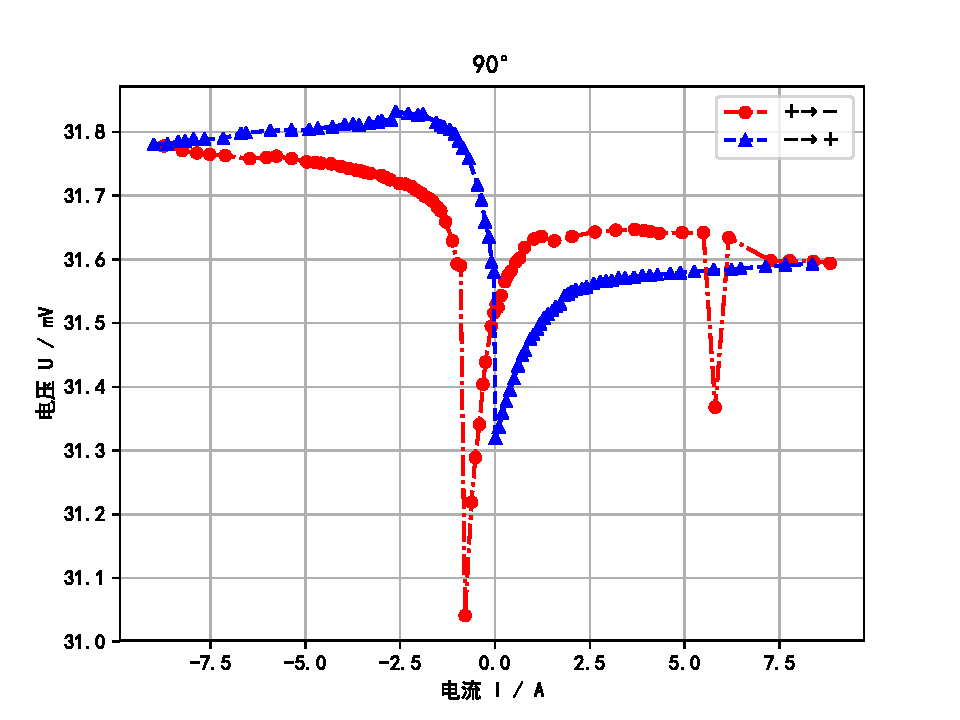
\includegraphics[width=1\textwidth]{fig/90.pdf}
\caption{平行方向数据图}\label{parallel}
\end{figure}

图(\ref{parallel})中有两个谷值,分别为31.041mV和31.32mV,取平均值为$U_{0\parallelsum}=$31.181mV;电流极值附近有两个电压饱和值,分别为31.78mV和31.594mV,取平均值为$U_{\parallelsum}=$31.687mV。

\subsection{垂直方向}
\begin{figure}[!h]
\centering
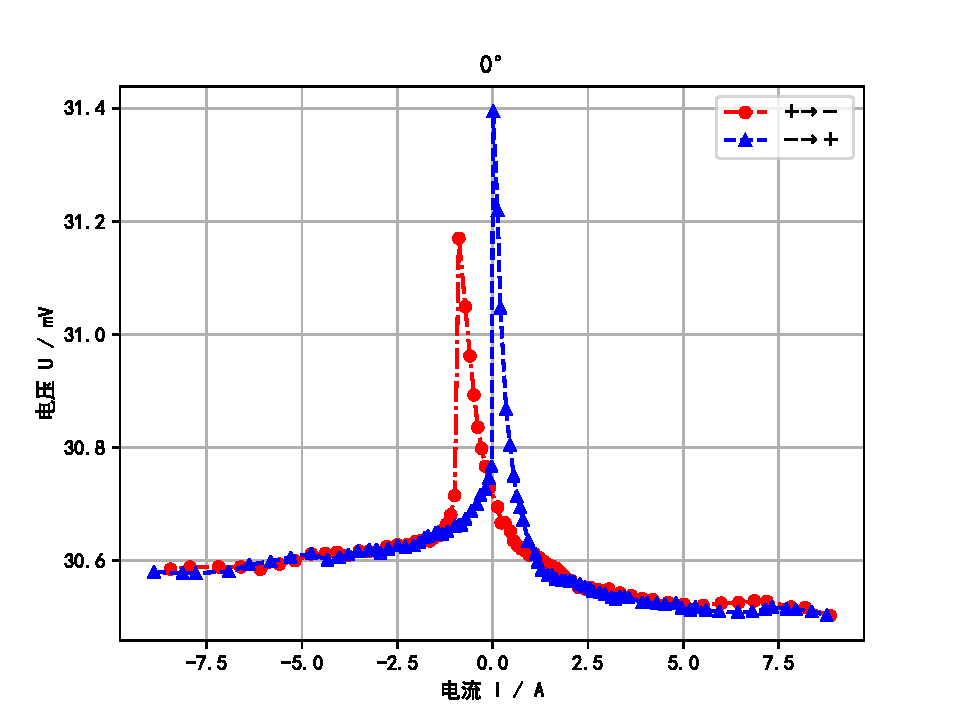
\includegraphics[width=1\textwidth]{fig/0.pdf}
\caption{垂直方向数据图}\label{perpendicular}
\end{figure}

图(\ref{perpendicular})中有两个峰值,分别为31.17mV和31.394mV,取平均值为$U_{0\perp}=$31.282mV;电流极值附近有两个电压饱和值,分别为30.58mV和30.503mV,取平均值为$U_{\perp}=$30.541mV。

\newpage
\subsection{计算AMR}
\begin{equation}
\text{AMR} = \frac{\Delta\rho_{\parallelsum} - \Delta\rho_{\perp}}{\rho_{0}} = \frac{U_{\parallelsum} - U_{\perp}}{U_{0}} = \frac{31.687 - 30.541}{\frac{31.181+31.282}{2}}\times 100\% \doteq 3.67\%\label{AMR}
\end{equation}

\section{误差分析}
\begin{enumerate}
	\item 实验方法。
	教材中要求我们从0开始增加亥姆霍兹线圈的电流,而我认为这样的方法是不妥的,%这是学长们被老师忽悠的方法!
	因为从0开始施加磁场,材料的磁畴可能仍处于杂乱状态,当磁场经历增大-减小-反向增大-减小的过程回到0时,材料的磁畴是处于有序状态的,即有剩余磁化,这样就和开始时测量的状态不一样。应该从磁场的极大或极小值开始测量。这也是图(\ref{parallel})和(\ref{perpendicular})中数据有一个极其陡峭的峰(谷)值的原因。
	\iffalse
	\item 仪器误差。实验中我们观察到实验所用的电压表有极其严重的漂移现象,放置一段时间按后同样环境的读数会增加0.1mV量级的偏差,而实验过程中我们读数时有一些停顿时间,这是实验数据误差的重要来源。
	\item 随着实验的进行,样品通电时间越来越长,产生的热量越来越多,可能导致样品温度发生变化,从而造成误差。
	\fi
\end{enumerate}

\section{思考题}
\subsection{测量AMR后计算出来的$\rho_{av}$和$\rho_0$是否相同,如不同说明什么问题?}
\subsection{按前述步骤手动测量的磁电阻曲线与自动测量的磁电阻曲线有何异同,为什么?}
\subsection{手动测量与自动测量时如何更好的选择流过样品的电流的大小?}
\subsection{测量中如何减小热效应对测量的影响?}
\subsection{样品夹具采用的材料有何要求?}

\nocite{jiaocai}
\bibliography{ref}
\end{document}